19. \begin{figure}[ht!]
\center{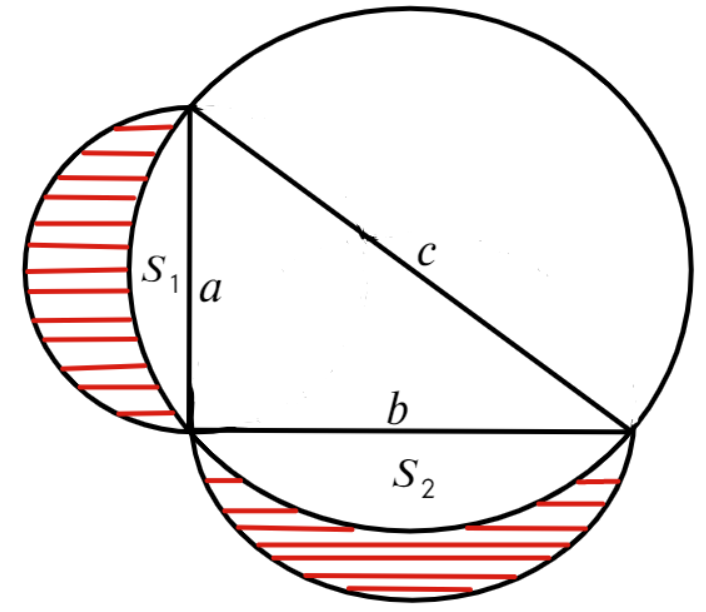
\includegraphics[scale=0.35]{g9-19.png}}
\end{figure}\\
Пусть катеты треугольника равны $a$ и $b,$ а гипотенуза --- $c.$ Искомая сумма площадей равна $\cfrac{\pi a^2}{8}-S_1+\cfrac{\pi b^2}{8}-S_2,$ где $S_1$ и $S_2$ --- площади сегментов, отсекаемых катетами треугольника от описанного круга. Выразим $S_1+S_2=\cfrac{\pi c^2}{8}-\cfrac{ab}{2},$ тогда
$\cfrac{\pi a^2}{8}+\cfrac{\pi b^2}{8}-(S_1+S_2)=\cfrac{\pi a^2}{8}+\cfrac{\pi b^2}{8}-\cfrac{\pi c^2}{8}+\cfrac{ab}{2}=\cfrac{a^2+b^2-c^2}{8}+\cfrac{ab}{2}=
\cfrac{ab}{2}=1.$\newpage\noindent
